
\begin{minipage}[c]{\textwidth}
\centering
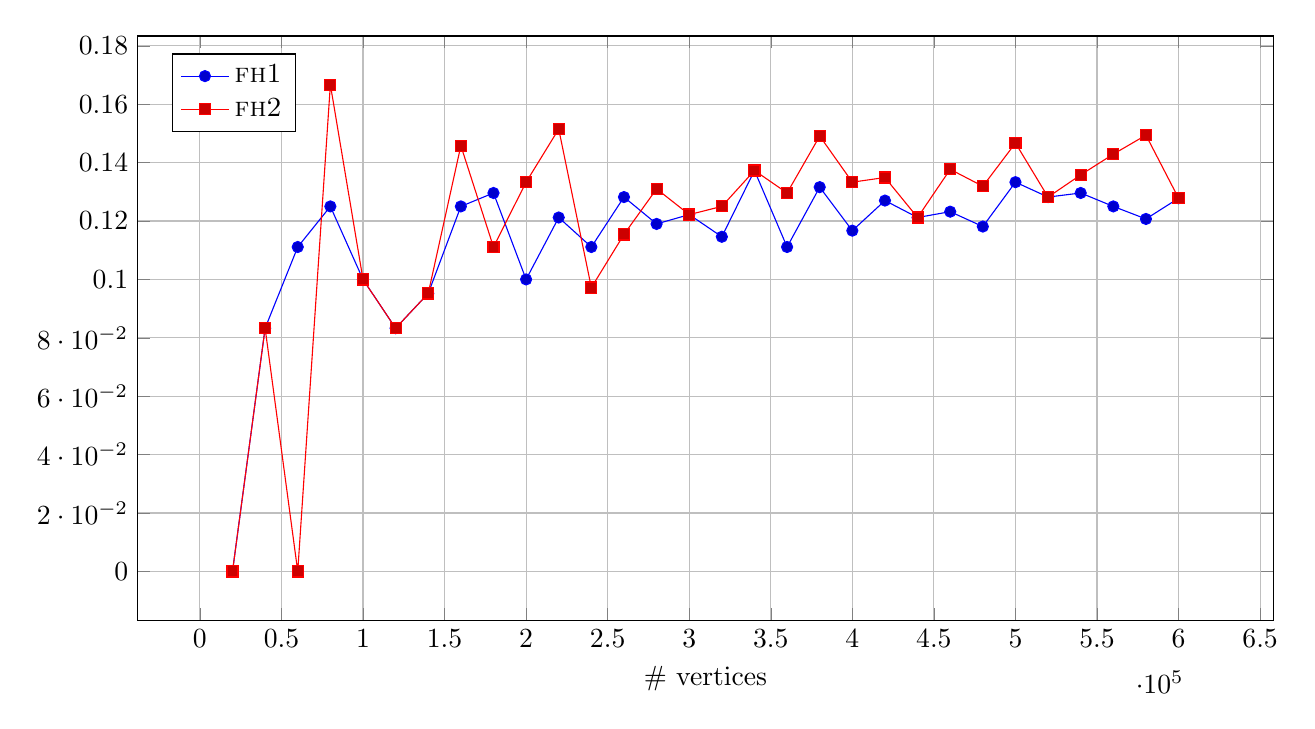
\begin{tikzpicture}
        \begin{axis}[
            xlabel = \# vertices,
            height=9cm,
            width=16cm,
            grid=major,
            legend pos=north west
    	]

        \addplot coordinates {
(20000,0.0000)
(40000,0.0833)
(60000,0.1111)
(80000,0.1250)
(100000,0.1000)
(120000,0.0833)
(140000,0.0952)
(160000,0.1250)
(180000,0.1296)
(200000,0.1000)
(220000,0.1212)
(240000,0.1111)
(260000,0.1282)
(280000,0.1190)
(300000,0.1222)
(320000,0.1146)
(340000,0.1373)
(360000,0.1111)
(380000,0.1316)
(400000,0.1167)
(420000,0.1270)
(440000,0.1212)
(460000,0.1232)
(480000,0.1181)
(500000,0.1333)
(520000,0.1282)
(540000,0.1296)
(560000,0.1250)
(580000,0.1207)
(600000,0.1278)

    	};
        
    	\addlegendentry{\textsc{fh1}}

        \addplot coordinates {
(20000,0.0000)
(40000,0.0833)
(60000,0.0000)
(80000,0.1667)
(100000,0.1000)
(120000,0.0833)
(140000,0.0952)
(160000,0.1458)
(180000,0.1111)
(200000,0.1333)
(220000,0.1515)
(240000,0.0972)
(260000,0.1154)
(280000,0.1310)
(300000,0.1222)
(320000,0.1250)
(340000,0.1373)
(360000,0.1296)
(380000,0.1491)
(400000,0.1333)
(420000,0.1349)
(440000,0.1212)
(460000,0.1377)
(480000,0.1319)
(500000,0.1467)
(520000,0.1282)
(540000,0.1358)
(560000,0.1429)
(580000,0.1494)
(600000,0.1278)

    	};
        
    	\addlegendentry{\textsc{fh2}}


        \end{axis}

    \end{tikzpicture}
    \captionof{figure}{Running time divided by $n$}
    \label{fig:time_14}
\end{minipage}
